%% The following is a directive for TeXShop to indicate the main file
%%!TEX root = diss.tex

\chapter{Introduction}
\label{ch:Introduction}
%Human beings are physical, social creatures, and our technology has only just started to communicate on our terms.
%Over the years, computing has progressed from symbolic, machine-focused communication like punch cards, assembly languages, and terminal interfaces to physical and natural user interaction.
%Yet despite embracing new interaction techniques like touchscreens and voice control, the rich senses of touch have been relegated to buzzing alerts or limited to high-stakes expert systems like laparoscopic surgery.
%
%Haptic technology involves the senses of touch; here we refer to both tactile (skin-based) and kinaesthetic (force- and position-based) perception.
%Between the resurgence of consumer virtual and augment reality (VR \& AR), rapid development of personal fabrication techniques, and recent additions of high-fidelity haptics to wearable products like the Apple Watch, we are poised to see haptic technology move from niche roles into mainstream adoption.
%This diverse field has been active in creating new devices and understanding human perception for decades, but the development of haptic media and design of haptic experiences remain a critical challenge.
%Haptic experiences are rich, diverse, multimodal entities which necessitate in-person interaction and have limited infrastructure.
%How can we enable creativity with these experiences?
%
%In this dissertation, I study the process of haptic experience design (``HaXD") and establish guidelines for building interactive software systems to support it.
%Through a series of implemented tools, we build pathways for haptic designers.
%This is complemented by both quantitative and qualitative inquiry to understand how haptic designers' experiences and their process.
%Critically, we examine contextual activities that are naturally supported in non-haptic design design, but break down when applied to touch-based interactions: sketching, editing, browsing, and sharing.
%
%
%\section{The state of haptic experience design}
%Haptics is great for many applications.
%Some of the highest profile benefits come from high-resolution medical contexts like remote surgery or dentistry simulation.
%More prevalent, wearables have opened up a wide variety of contexts for unobtrusive tactile feedback, such as exercise bands.
%Accessibility remains an important use for touch-based technology for when other modalities are unavailable.
%Affective display, like communicating the emotions of a loved one, can take advantage of the personal nature of touch.
%%VR \& AR
%
%Of course, lots of work has gone into understanding how to make effective haptics.
%Design guidelines tell us effective ways to communicate large sets of information, provide spatial guidance, and even how to perform tactile concerts.
%% tactile icons and tactons to more sophisticated affective qualities ...
%Several editors and design tools have been built to create
%However, they don't consider the wider context of design: the fact that creativity is a social process that takes place in our environment, where designers build upon new ideas, receive feedback from others, and incroporate their personal experience into their designs.
%
%
%
%
%\section{Creativity in context}
%A painter snatches her paintbrush, sets her easel, and begins.
%An image of \emph{La Grande Jatte} slowly emerges, one stroke at a time, each colour carefully considered.
%What is missing from this scene?
%First, the landscape: is it laid out in front of our painter, referenced from a photograph, remembered, or purely imagined?
%Does she stand alone, or is there a friend giving an impression?
%How does she feel on this particular day, and is she painting for fun or money (or both)?
%
%In this dissertation, I make a simple argument: context must be considered for creative tasks. I then apply this argument to haptic experience design.
%The central goal is arguing for an embodied process of design, a systems model of design. This is applied to both a single haptic experience (consider hardware, user, etc. and all the challenges that this system entails), and to the designer?s process, situated in customers, colleagues, examples, and the design right in front of her.
%
%Many people have argued that creativity is not a solitary endeavor; Mihaly (cite), Warr (cite), shneiderman (...). Buxton, ... .
%Recent design research has empirically evaluated this ... Kellmmer, Dow, Hartmann, ... .
%
%Ultimately, creativie interfaces must have low-bar, wide walls, high ceiling; haptic desogn has none of these.
%
%
%
%\section{The difference of haptics}
%By applying advanced design and creativity thinking to haptics, we find two things: 
%1) a way to further improve haptic design, empowering designers, developers, and end-users to create for this new field, and 
%2) a confirmation and elaboration on design thinking.
%Many ideas that are taken for granted in graphic design break down when applied to haptics. 
%This makes us think more critically about design and creativity, and can inform other fields by showing us how haptic experience design is different, and supporting design processes for other, future technologies that are still emerging. (Examples ???)
%
%
%\section{Approach and Contributions}
%describe methodology - design working tools, study process, design extra toools, design haptics, and talk to designers from ground up.
%Multi-pronged approach to understanding this problem.
%
%List of chapters here:
%
%
%
%\osC{bookmark}
Haptic sensations enable engaging, personal, and low-attention experiences, but this is limited due to little support for \emph{designing} a haptic sensation.
Computer-controlled haptic experiences are a recent phenomenon; the focus on technology requirements and rapidly changing field has left little room for examining processes of design in a methodical way.

While many tools exist to support design in other modalities, such as graphic design, there are few for haptics.
Part of this comes from immaturity of the field and lack of market penetration of highly expressive haptic devices.
However, there are also intrinsic challenges to designing for the sense of touch.
I want to develop practical tools that support the HaXD process, building a body of knowledge of how to facillitate this difficult subfield of design.
I approach this problem with two different strategies:
\begin{enumerate}
\item \textbf{Vibrotactile design case studies.}
To understand design, I take a design perspective.
In each of three case studies, I design, build, and evaluate a tool to support an aspect of haptic experience design, scoped to \emph{vibrotactile} (VT) design.
Each of these results in concrete implications for designing tools and a small window onto the larger HaXD process.
Contributions include algorithms, data structures, interaction techniques, features, and working software tools that have been employed by designers.
\autoref{ch:hapticinstrument}, \autoref{ch:hapticanimation}, and \autoref{ch:hapticexamples} outline these.

\item \textbf{Synthesis into preliminary theory.}
While the case studies provide an in-depth investigation into vibrotactile sensation design, results may not generalize to other devices.
Furthermore, despite the recent growth of the field, haptic designers remain relatively rare and difficult to recruit.
To generalize our findings to other situations and ground it with haptic experience designers, I plan to draw from other data sources: a workshop held at World Haptics 2015, already-collected interviews with haptic designers, and a number of side-projects.
This synthesized contribution will help refine our findings, such as tasks, goals, barriers, strategies, and practices designers use and face when working with haptics.
\end{enumerate}


\begin{figure}[htbp]
\begin{center}
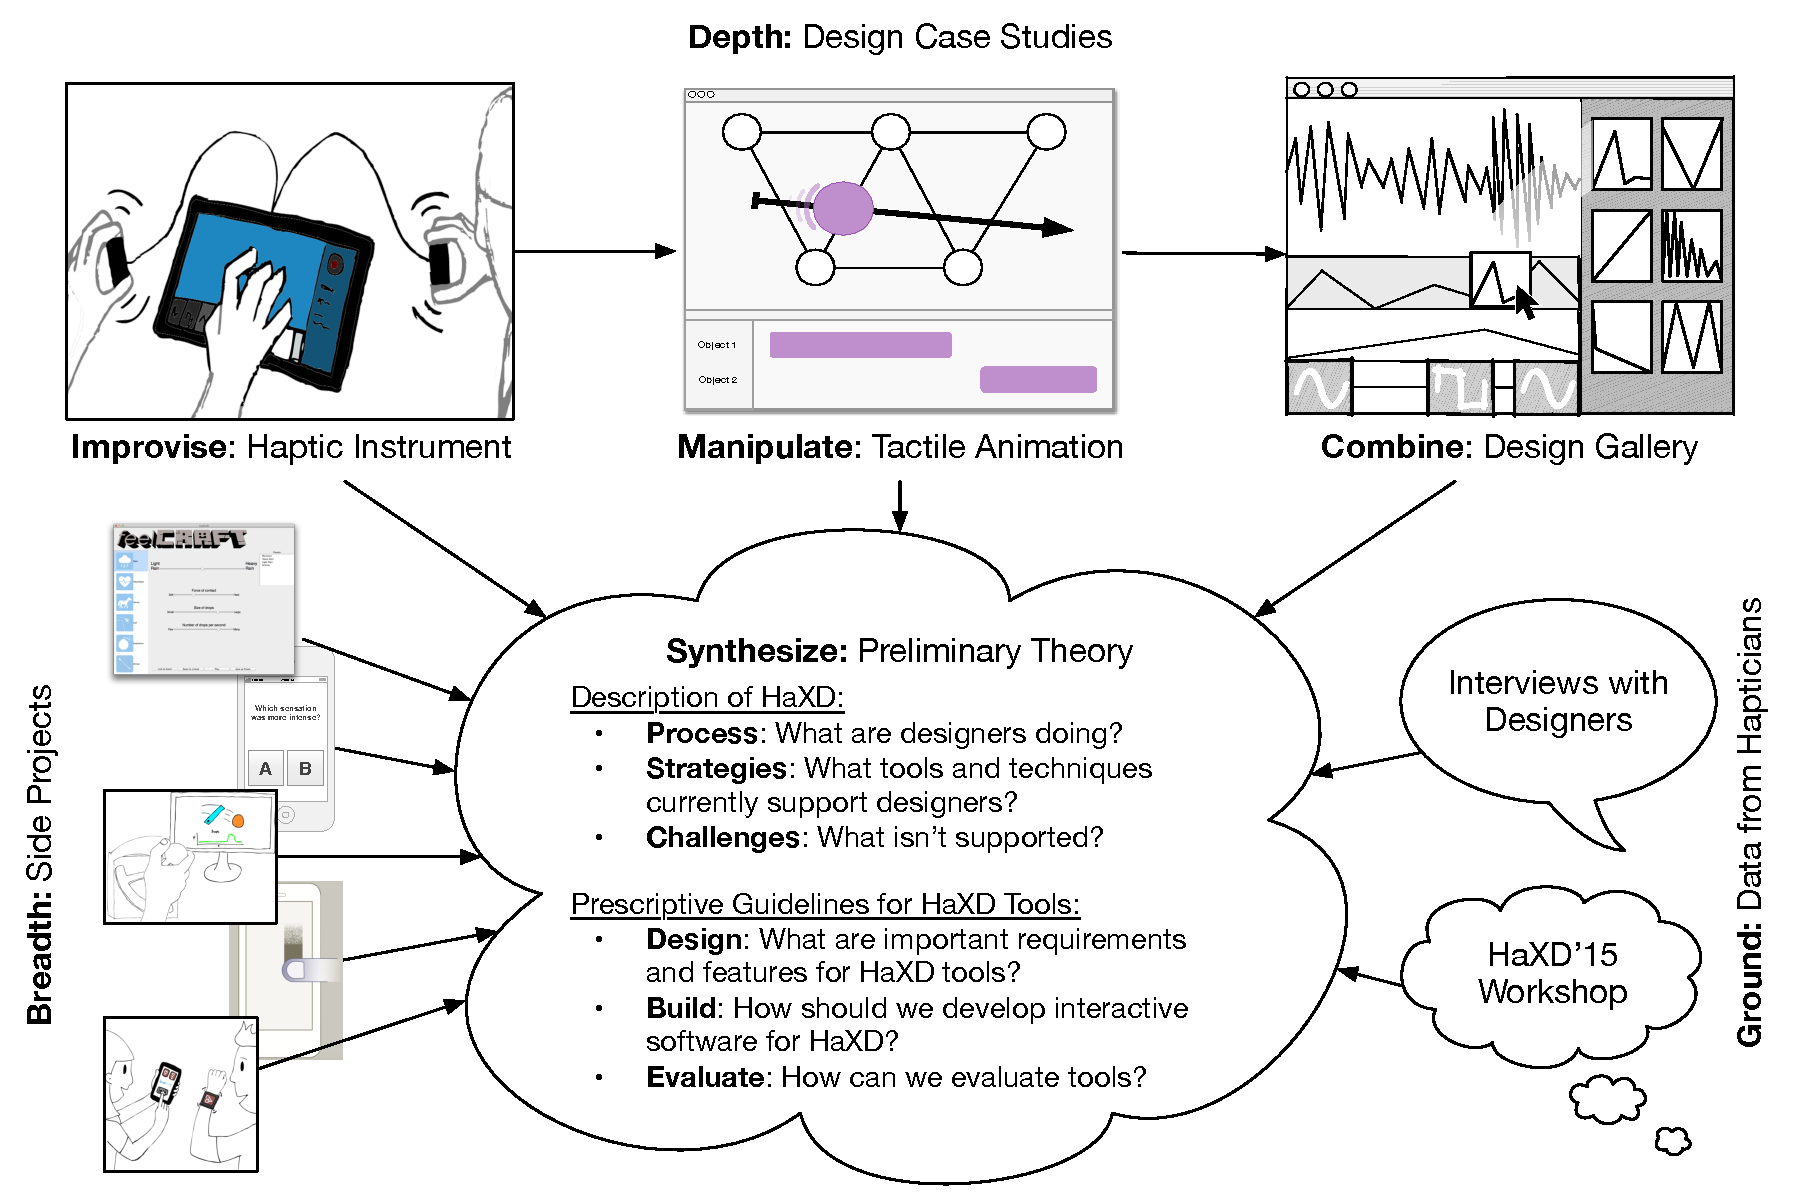
\includegraphics[width=\textwidth]{HaXDTheoryOutline-2015-05-22}
\caption{Methodology overview. Three case studies investigate VT tools in-depth; findings are synthesized with side projects and grounded data into a preliminary theory.}
\label{fig:intro:methodologyoverview}
\end{center}
\end{figure}


\section{Vibrotactile Design Case Studies}

Each case study investigates a different set of design concepts with varying user populations, VT device, and design challenges (\autoref{fig:intro:casestudyoverview}), but restricts scope to VT sensations.
This offers a deep look into an expressive and increasingly common class of haptic devices, allowing us to explore critical features in a somewhat controlled fashion.
An iterative approach allows us to refine ideas and methods, and so each case study follows three steps: \emph{gather}, finding requirements and previous design elements; \emph{create}, where we design and build the tool; and \emph{evaluate}, where we test the tool with its target population and consolidate lessons learned.

In Study 1, the Haptic Instrument, we focus on real-time, rapid design of VT sensations with a first look into themes of real-time design and collaboration.
When participants worked with our tool, mHIVE (a ``mobile Haptic Instrument for Vibrotactile Exploration"), compositions couldn't be edited, suggesting mHIVE was suitable for exploration and improvised communication, but not as suited to refining ideas.
This informed Study 2, Tactile Animation, where we developed a single abstracted animation object directly manipulated in both space and time.
Animators found our tactile animation tool, Mango, easy-to-use, and confirmed our findings about the value of real-time exploration.


\begin{figure}[htbp]
\begin{center}
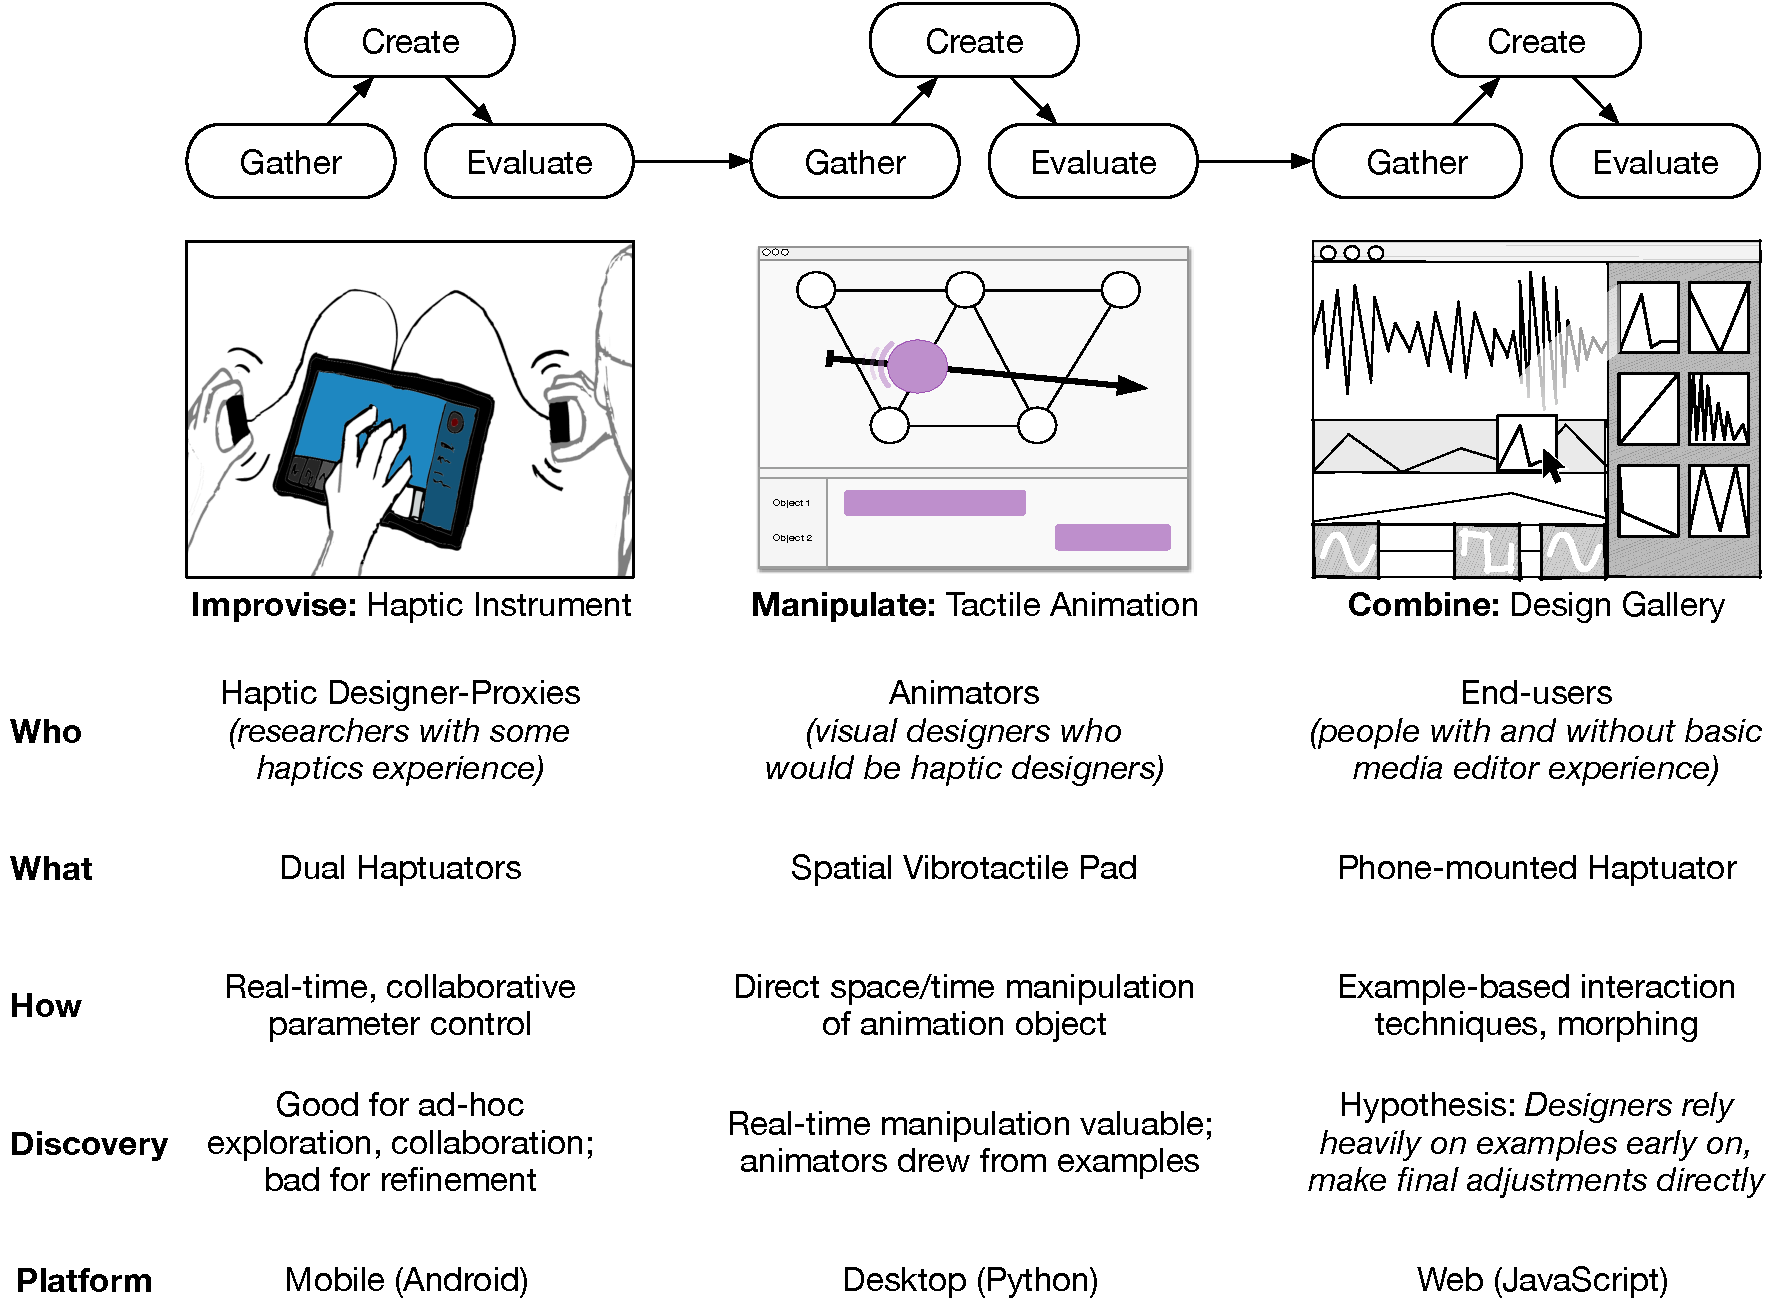
\includegraphics[width=\textwidth]{HaXDTheoryCaseStudyOutline-2015-05-28}
\caption{Vibrotactile design case studies. Each studies an aspect of vibrotactile design with a varied set of users, devices, platforms, and foci.}
\label{fig:intro:casestudyoverview}
\end{center}
\end{figure}

One stand-out result from both Mango and mHIVE is that designers drew from their experience or examples found in the world, and wanted to re-use what they had created (e.g., through copy and paste).
In Study 3, I explore the role of examples in haptic design.
This study is codenamed ``Project Macaron" and consists of two phases.
Phase I, ``algorithms and interaction techniques", builds a set of perceptually-verified ways to manipulate examples and incorporate them into designs.
In Phase II, we use the results of Phase I to create a haptic design gallery interface, and study how and when users incorporate examples into their VT designs.
In this way we hope to consolidate our findings from mHIVE and Mango, and capture our participants' design process more concretely through logging of user actions.

These studies are described in more detail in \autoref{ch:hapticinstrument},  \autoref{ch:hapticanimation}, and \autoref{ch:hapticexamples}.
Each chapter is presented as an outline of what will appear in the final dissertation, summarizing methods and results for completed work and outlining planned work.


\section{Synthesis of Contributions}

Each case study provides concrete knowledge for building a vibrotactile authoring tool, and some insight into the vibrotactile design process.
However, haptic technology consists of many devices and experiences beyond vibrotactile.
%In addition, it is difficult to find and recruit haptic designers.
I will synthesize findings from the three design case studies together with a number of side projects, the design literature, community feedback from a workshop on haptic experience design, and interviews with haptic designers into a preliminary design theory on how to support the creation of engaging, captivating haptic experiences.
I expect to make progress on the following questions:
\begin{enumerate}
    \item \textbf{Description of the Haptic Design Process.}
    What are the major \textbf{processes and tasks} conducted by haptic designers?
    What \textbf{strategies} do haptic designers employ, including existing tools?
    What are the \textbf{challenges} haptic designers face?
    
    
    \item \textbf{Prescriptive Implications for HaXD Tools.}
    What are major \textbf{requirements} and \textbf{features} for designing HaXD tools?
    What are some considerations when \textbf{implementing} HaXD tools in software?
    How can we \textbf{evaluate} design tools effectively?
\end{enumerate}

This process is described in \autoref{ch:haxd}.


\section{Summary of Progress}

I am currently working on the \emph{create} stage of the third case study; the first two have papers either published or in peer-review.
Multiple side projects are underway, primarily  carried out by undergraduate students I'm co-supervising.
All side projects are expected to be substantially developed or completed by the end of summer 2015; the FeelCraft side project has already been published and presented.
For more information on current progress, please see \autoref{ch:timeline}.


The proposal continues as follows.
First, in \autoref{ch:rw}, I cover related work with an overview of haptic technology and applications, a presentation of existing haptic design tools, and a discussion of design theory from other fields.
Then, I outline each VT design case study in \autoref{ch:hapticinstrument},  \autoref{ch:hapticanimation}, and \autoref{ch:hapticexamples}.
%Each chapter is presented as a direct outline of what will appear in the final dissertation, summarizing either methods and results (\autoref{ch:hapticinstrument} and \autoref{ch:hapticanimation}) or proposed methods and possible results (\autoref{ch:hapticexamples}).
After, I describe the planned data synthesis in more detail in \autoref{ch:haxd}.
Finally, I present milestones and a timeline for my PhD in \autoref{ch:timeline}.


\section{Contributions}

In \autoref{ch:hapticinstrument}, we present findings from our first vibrotactile design tool, the haptic instrument, which supported easy exploration and informal feedback, but identified a key problem: lack of refinement for designs.

In \autoref{ch:tactileanimation}, we present findings from our second vibrotactile design tool, Mango, which established a generalized pipeline and was able to support both exploration and refinement for expert visual animators; it highlighted reuse as an important next step.

In \autoref{ch:macaron}, we present findings from our third vibrotactile design tool, Macaron, which implemented a browsing interface and analytics system; we found examples played a large part of the design process, and that a web-based tool allowed for easy deployment.

In \autoref{ch:hapturk}, we document findings from HapTurk, a technique for getting feedback on vibrotactile designs at scale: from the crowd using proxy vibrations distributed over Mechanical Turk; we also comment on uses for haptic broadcasting.

In \autoref{ch:sideprojects}, we synthesize together findings from our side projects, showing generality by applying our understanding of haptic design explicitly in several domains and gaining practical experience designing haptic experience.

In \autoref{ch:hapticianinterviews}, we complement our design-based inquiry through interviews with professional haptic designers and a workshop run to elicit feedback from the community; this captures a description of haptic design, reinforcing our findings for important support tools, and identifies more systematic challenges.

Finally, in \autoref{ch:conclusion}, we conclude with a summary of our final results and directions for future research.


%
% END
%
\endinput

Any text after an \endinput is ignored.
You could put scraps here or things in progress.
